\chapter[Linear ICS at Astra Gemini]{Linear Inverse Compton Scattering at Astra Gemini}
\label{Chap:linICS}
                                                                                                                                                                                                                                                                                                                                                                                                                                                                                    \section{Motivation}

Linear Inverse Compton scattering has been widely used as high-energy radiation source to study nuclear processes, diagnose beam properties (energy, emittance, polarisation) and recently in laser wakefield accelerators as source for imaging applications.

As lasers are more intense we now also access the regime where we can use linear ICS as a single-shot diagnostic.

In the context of radiation reaction studies, linear ICS, especially in the transient regime between linear and non-linear is useful to characterise electron beams and estimate the fluctuations.

If the gamma detector is sensitive enough this could also be used to estimate the intensity by considering the nonlinearity.

\section{Chapter Outline}



\section{Experimental Setup}

This experiment was performed at the Gemini facility in early 2019 using both laser arms of the dual laser beam facility.
A sketch of the relevant components of the setup are shown in Figure \ref{LinICS:Fig:SetupBlend}.

\begin{figure}
\centering
\includegraphics[width=0.9\columnwidth]{GeminiShock2019_ExpBlend_V1_Aug20_annotated.png}
\caption[Sketch of experimental setup to measure radiation from linear inverse Compton scattering.]{Sketch of the experimental setup aimed to measure radiation from linear inverse Compton scattering. The first laser pulse (red, left) is focused down by an $f/40$ OAP into a gas jet and accelerates electrons (blue) from LWFA, where the density perturbation induced by the blade affects the injection mechanism. A second laser is focused down by an $f/2$ OAP and counter-propagates with the electron beam performing linear inverse Compton scattering. Gamma radiation produced in the interaction (green) is emitted in the propagation direction of the electron beam and is measured downstream by a scintillating profile screen and a stack of scintillating crystals used as spectrometer (right). A converter target behind the $f/2$ OAP can be used to convert the electron beam via bremsstrahlung into an energetic calibration source for the gamma diagnostics. The electrons are dispersed horizontally by a permanent dipole magnet onto a set of Lanex screens. The accelerator, the interaction point and the magnet are in vacuum, whereas the measurement screens and gamma diagnostics are located at air separated by a thin vacuum window (orange).} 
\label{LinICS:Fig:SetupBlend}
\end{figure}


\subsubsection{Laser wakefield accelerator}

The driver beam for the wakefield accelerator is focused by an $f/40$ off-axis parabola (OAP) onto the leading edge of a 15 mm conical supersonic helium gas jet. The measured pulse duration was $61\,\mathrm{fs}$ \textsc{fwhm} with an average energy on-target of $12.5 \pm 0.2\,\mathrm{J}$, reaching a peak power of $195\,\mathrm{TW}$. The size of the focal spot measured $48.6 \times 39.2\,\mathrm{\mu m}$ \textsc{fwhm}, amounting to a peak normalised vector potential of $a_0 = 1.88$ in vacuum\footnote{The focal spot and FROG trace were analysed by Matthew Streeter (Imperial College)}. The laser is polarised in the horizontal plane.
\vspace{\baselineskip}

The exit of the gas nozzle was positioned $14\,\mathrm{mm}$ below the laser beam axis to avoid damage from the second, more divergent laser beam. A steel razor blade is introduced $4\,\mathrm{mm}$ above the nozzle edge at $- 32.4\pm 0.3^\circ$ angle in vertical direction relative to the laser axis to produce a shock front. The tip of the blade is inserted $1.2\,\mathrm{mm}$ into the gas flow from the same side that the driver beam enters from. 
The gas target was characterised on-shot by a transverse optical probe synchronised with the driver beam ending in a shadowgraphy and a Mach-Zehnder interferometry setup.
The interferometrically determined electron density\footnote{The interferometry data was evaluated by Cary Colgan (Imperial College)} without inserting the blade was $(1.4 \pm 0.2) \times 10^{18}\,\mathrm{cm}^{-3}$. When inserting the blade the density profile exhibits a sharp peak in density reaching about $(2.4 \pm 0.2) \times 10^{18}\,\mathrm{cm}^{-3}$, which is about twice the ambient density.

The gas target and the recombination light emitted by the plasma channel are imaged by a Canon DSLR camera from the side and a CCD camera from the roof of the chamber.

\subsubsection{Scattering beam}

A second laser pulse is focused by an $f/2$ off-axis parabola (OAP) at the opposite edge of the gas jet in a head-on geometry. The $f/2$ OAP has a 21-mm-diameter hole in the centre that allows the electrons, laser light and radiation to propagate through. A plastic ring of outer radius $28\,\mathrm{mm}$ and inner radius $11\,\mathrm{mm}$ is fitted around the hole to protect the optic and the laser chain upstream from potentially in the plasma scattered or strongly defocused driver laser light. This reduces the on-target intensity by 16 percent assuming a perfect top-hat laser profile and that the collimated beam incident on the OAP has a diameter of $150\,\mathrm{mm}$. To protect the optic from potential debris a thin plastic layer with anti-reflective coating (`pellicle') and a suitable hole is attached to the mount of the OAP. The on-shot energy of the laser after the compressor was $9.73\pm 0.15\,\mathrm{J}$ and $8.17\pm0.13\,\mathrm{J}$ on-target due to the hole in the OAP. In the dataset presented, the beam size is defocused to a spot of about $400\pm50\,\mathrm{\mu m}$ diameter, which translates into $a_0 \sim 0.28 \pm 0.03$ at the interaction. The laser is linearly polarised in the vertical plane, cross-polarised to the wakefield driver beam.

\subsubsection{Two-beam timing}

Both laser beams are synchronised to each other using spatial interferometry \cite{Cole2018_RR}. A 90-degree dielectric knife-edge prism (Thorlabs MRAK25-E03) was inserted at the interaction point, deflecting both beams collinearly onto the CCD chip of a camera (AVT Manta G-033B) equipped with a X10 long-working-distance infinity-corrected microscope objective. Due to the different radii of curvature of both beams, especially near the focus of the $f/2$ beam, a circular interference pattern emerges when the beams are overlapped in space and time. The timing procedure is explained in more detail in the \nameref{Chap:Methods}.

\subsubsection{Particle and Radiation diagnostics}

The radiation, the remaining driver laser and the electrons propagate through the hole in the $f/2$ OAP into a large aperture ($10\,\mathrm{cm} \times 30\,\mathrm{cm}$) permanent dipole magnet\footnote{designed, and assembly and positioning supervised by Dominik Hollatz (Jena)} of integrated magnetic field strength $\int B(x) \mathrm{d}x = 0.35\,\mathrm{Tm}$. 

The electrons are dispersed in the horizontal plane and electrons of energy lower than 220 MeV collide with the yoke of the magnet resulting in an effective low-energy cut-off. The dispersed beam leaves the vacuum chamber through a two-layer wide-aperture vacuum window\footnote{designed and tested by the Mechanical Engineering Division at the CLF, in particular Daniel Treverrow.} of dimensions $580 \,\mathrm{mm} \,\times\, 70\,\mathrm{mm}$ (horizontal $\times$ vertical). The layer facing the vacuum consists of $25\,\mathrm{\mu m}$ of Kapton, the outside layer is $375\,\mathrm{\mu m}$ of Kevlar providing additional mechanical stability and fibre support that acts as fail-safe. A scintillating sensitive Lanex (Kodak Biomax) screen placed just after the window, at $1.61\,\mathrm{m}$ distance downstream of the interaction point, measures the spectrum of the dispersed electron beam. The screen also extends beyond the laser axis. The light and thin material of the window and the short distance to the Lanex screen minimises the impact of small-angle scattering on the measurement (REF MOLIERE SCATTERING).
A second standard Lanex screen measures the spectrum $700\,\mathrm{mm}$ further downstream ($2.31\,\mathrm{m}$ from the interaction point) and can in conjunction with the first screen be used to account for the pointing of the beam \cite{Soloviev2011_TWOSCREEN}.
The screens are each imaged by a cooled 16-bit CCD camera (Andor Neo) equipped with suitable objective and bandpass filter. %A third camera images a small region of interest on the first screen.
\vspace{\baselineskip}

High-Z metal converter targets (bismuth, tungsten) fixed to a $1.6\,\mathrm{mm}$ plastic (PTFE) base are mounted on a motorised linear stage between the $f/2$ OAP mount and the dipole magnet, and can be driven into the beam path to intercept the electron beam and to produce gamma radiation from bremsstrahlung \cite{Glinec2005_Brems}. This is used to calibrate the gamma-ray diagnostics in this experiment \cite{Behm2018_Gamma}. The high-Z targets are expected to enable efficient conversion of the electron beam energy into radiation, but do not allow measuring the electron spectrum at the same time. The PTFE base itself can also be used as converter that is less efficient in terms of radiation yield but allows a synchronous measurement of the electron and gamma-ray beam. 

Radiation traverses the magnet on the laser axis, then passes through a $120\,\mathrm{\mu m}$ aluminium laser beam block terminating the wakefield driver beam and the Kevlar-Kapton window mentioned before. Bright radiation in the right bandwidth is also captured by the Lanex screen as it extends beyond the laser and radiation axis. An array of $45 \times 45$ scintillating with thallium doped caesium-iodide (CsI:Tl) crystals coated in $TiO_2$ of dimensions $1\,\mathrm{mm} \times 1\,\mathrm{mm} \times 10 \,\mathrm{mm}$  measures the profile of the radiation $700 \pm 1\,\mathrm{mm}$ downstream from the plane of the first Lanex screen. The stack covers a field of view corresponding to a cone of half opening angle $11.7\,\mathrm{mrad}$. The spatial resolution including the coating separating the individual crystals is then $1.2\,\mathrm{mm}/2.31\,\mathrm{m} = 0.52\,\mathrm{mrad}$. %A scintillation signal produced by radiation on the first Lanex screen and the CsI profile screen can be used as on-shot reference for the laser axis for the electron spectrometer screens. 
$704 \pm 1\,\mathrm{mm}$ further downstream from the profile screen another elongated array of caesium-iodide crystals is positioned to measure the spectrum of the gamma radiation. Both scintillator arrays, the profile screen and the spectrometer, are imaged using cooled 14-bit EMCCD cameras (Andor iXons). The diagnostics are described in more detail in the \nameref{Chap:Methods} section.

\iffalse
The aperture of the magnet permits a field-of-view of $79\,\mathrm{mrad}$ (10cm/1.26m) and is hence less limiting than the OAP hole. On the laser axis a beam block of $10-12$ layers of standard kitchen aluminium foil of thickness $10.1 \pm 0.2 \,\mathrm{\mu m}$ each is attached to the Kevlar-Kapton window. Hard X-rays continue to propagate through the aluminium beam block and the vacuum window (permitting a FOV of $70/1.61 = 43.4 mrad$ , the LANEX screen that also covers the axis and are then after $700\,\mathrm{mm}$ incident on a $45 \times 45$ array of $1\,\mathrm{mm} \times 1\,\mathrm{mm} \times 10 \,\mathrm{mm}$ scintillating caesium-iodide crystals coated in $TiO_2$ that record the beam profile of the radiation burst. The top part of the stack is centred on the beam axis. The total stack covers $54.2/2.31 = 23.4\,\mathrm{mrad}$. A second $30 \times 30$ stack of  $1.5\,\mathrm{mm} \times 1.5\,\mathrm{mm} \times 10 \,\mathrm{mm}$ CsI crystals is placed on top of the other one, covering another $51.2\,\mathrm{mm}$ or $22.2\,\mathrm{mrad}$. Harder radiation propagates another $704\,\mathrm{mm}$ before hitting another array of caesium-idodide crystals (see Methods for dual axis spectrometer) with an aluminium front-plate that are arranged in longitudinal direction to measure the spectrum of the radiation. The front part of the spectrometer then catches $XX/3m$ FOV. The emission of the caesium-iodide crystals is imaged by Andor iXon cameras.
\fi

\section{Characterisation of Electron Spectra}

The electron beams from laser wakefield acceleration were in this experiment injected by density perturbations in the supersonic gas flow which were introduced by a steel blade. The spectrum is measured by scintillating Lanex screens as part of a magnetic spectrometer setup. The image processing of the data is not further elaborated here but can be found for instance in \cite{ColeThesis,PoderThesis} or the \nameref{Chap:Methods} of this thesis. We will only consider the first Lanex screen and ignore errors in the inferred electron energy due to global pointing.

We consider a dataset consisting of a series of shots at fixed conditions to investigate fluctuations in the accelerator performance. These electron beams were collided with the laser pulse and will in the following analysed in more detail for ICS.

The dataset consists of 386 shots with electron beams, taken at constant backing pressure of the gas jet and fixed blade position (1.2 mm into the gas flow from the entry point of the driver beam). A waterfall plot of the in non-dispersion direction integrated electron spectra is shown in \ref{linICS:Figs:fixed_waterfall}. Despite the constant conditions, the properties of the electron beams vary strongly from shot-to-shot and produce beams of a wide range of shapes, maximum energy and energy spread. A few examples of electron spectra from the dataset are provided in Figure \ref{linICS:Figs:Elec_example}.
The spectral length of the beams varies strongly with some starting below the measurement threshold of 220 MeV with significant amount of charge all the way up to 1 GeV, stretching 800 MeV of spectral range (see for instance the two panels on the left and right in Figure \ref{linICS:Figs:Elec_example}). These spectrally very wide electron beams show signatures of strong transverse oscillations which indicate potential to act as a bright betatron source (REF). In other instances beams with narrow energy spread around 1 GeV are measured (central panels in Figure \ref{linICS:Figs:Elec_example}). 


\begin{figure}
\centering
\includegraphics[trim={4.0cm 0 5cm 0}, clip, width=1.0\columnwidth]{Example_Montage_twoSets.png}
\caption[Waterfall plot for electron spectra at fixed conditions.]{Waterfall plot of electron spectra measured at fixed experimental conditions. The y-axis indicates the electron energy in MeV, the x-axis shows the order the shots were taken. The electron spectra measured on the Lanex screens were integrated in the non-dispersion axis and each occupy one column in this waterfall plot. The colour scale indicates the charge per MeV in the beam.}
\label{linICS:Figs:fixed_waterfall}
\end{figure}


\begin{figure}
\centering
\includegraphics[trim={4.8cm 0 5cm 0}, clip, width=1.0\columnwidth]{Example_Espec_CollisionMontage.png}
\caption[Examples of 2D electron spectra measured in the experiment.]{Examples of 2D electron spectra measured in the experiment. The y-axis is the dispersion axis and shows the electron energy in MeV on a linear scale, the x-axis indicates the divergence in mrad. The colour scale indicates the amount of charge per MeV per mrad in the beams and is fixed for all plots. Projections of the beams are shown on the respective axes: on the x-axis the over the dispersion-axis integrated spectrum is shown and is equivalent to the horizontally integrated spatial profile of the beam and is shown as charge per mrad as a function of divergence in mrad. The projection on the y-axis is the in non-dispersion axis integrated spectrum as also shown in the waterfall plot in Figure \ref{linICS:Figs:fixed_waterfall} and shows the charge per MeV as a function of the electron energy in MeV. The amplitude of the projections is fixed across all panels and is not representative of the relative charge between the panels.}
\label{linICS:Figs:Elec_example}
\end{figure}

The striking variability of the electrons produced in this dataset at seemingly fixed experiment conditions is not consistent with experimental results reported from other LWFA experiments at other laser systems using shock injection (REF). These setups typically provide reproducible electron beams with narrow energy spread (REF). 
\vspace{\baselineskip}

\begin{figure}
\centering
\includegraphics[trim={6cm 0 6cm 0}, clip, width=1.0\columnwidth]{linICS_ElectronProperties_Histograms.png}
\caption[Histogram of fluctuations in the electron beam properties in this dataset.]{Histograms showing the fluctuations of electron properties in course of this dataset (386 shots). Top left: Total charge of the electron beams measured from 220 MeV upwards. Top right: Maximum electron energy, defined as energy at which the spectral intensity falls to 10 percent of its peak value. Bottom left: FWHM Vertical divergence (non-dispersion axis) in mrad. Bottom right: Beam pointing fluctuation in mrad from the mean position. }
\label{linICS:Figs:Elec_histogram}
\end{figure}

The key properties of the electron beams in this dataset are summarised in Figure \ref{linICS:Figs:Elec_histogram} in form of histograms showing charge, maximum electron energy, vertical (non-dispersion axis) divergence and beam pointing.
The maximum energy of the electron beam, here defined as the energy when the spectral intensity reaches 10 percent of its peak value, was measured to be $944\pm139\,\mathrm{MeV}$, with some shots reaching up to 1.3 GeV. The charge of the beam varied in particular due to the varying spectral range of the bunch with a mean of $239 \pm 92\,\mathrm{pC}$.
The divergence of the beams was measured to be $2.7\pm 2.5\,\mathrm{mrad}$ and the vertical position of the beam centroid was fluctuating by $2.2\,\mathrm{mrad}$.
\vspace{\baselineskip}

The wide range of electron beams produced in this setup is interesting in the context of radiation production by linear inverse Compton scattering (ICS). Since the properties of the beams this accelerator is able to produce vary strongly, the radiation they produce in a well-defined linear ICS interaction will also vary significantly. This means that this accelerator is in principle also able to produce a wide range of radiation spectra from broadband to strongly peaked radiation, but we would need to increase the control over the accelerator to be able to select the right spectral shapes for the respective application. 


\section{Laser raster scan}

\begin{figure}[h]
\centering
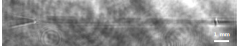
\includegraphics[width=0.8\columnwidth]{RasterScan_Shadowgraphy_CloseUp.pdf}
\caption[Shadowgram of the plasma channel with the focusing f/2 laser cone.]{Cut-out of a shadowgram taken with the transverse optical probe (horizontal plane) of the gas jet. The wakefield driver beam enters the gas jet from the right side and generates a plasma channel. The dark line on the right side results from a shock front. The second scattering beam is focused tightly into the plasma from the left side, where a converging cone becomes visible.}
\label{linICS:Figs:ShadowgraphyRaster}
\end{figure}

We followed an alignment procedure to overlap the two laser beams in space and time using a photodiode and spatial interferometry in a low power pulsed laser mode. The scattering beam is focusing into the plasma and is on full-power shots visible on the transverse (horizontal plane) shadowgraphy diagnostic (see Figure \ref{linICS:Figs:ShadowgraphyRaster}, left side) also showing the plasma channel from the wakefield driver beam and the shock leading to the injection of electrons into the wakefield accelerator (dark line in the plasma channel on the right side). Another camera is used to image the self-emission of the plasma from the vertical plane (top view).

On full-power shots with both laser beams and an electron beam produced in the wakefield accelerator, we consistently measured a bright circular or oval signal on the gamma profile screen. The consistency of the collisions indicates that the laser beam is larger than the electron beam and any fluctuations in the relative position of scattering beam and electron beam.

To establish the transverse size of the scattering laser pulse at the interaction point, we translated the scattering laser beam in one transverse axis by translating the position of the $f/2$ OAP. During this we keep the experimental parameters and the alignment of the wakefield driver beam fixed. At each OAP position we took 5 full-power shots with both laser beams firing and an electron beam being measured. More shots were taken if one of the lasers failed to shoot or no electron beam was measured to accumulate 5 suitable shots. The response of the gamma profile screen was recorded and the number of visible bright signals was noted down. The OAP was then translated by 50 microns and the procedure was repeated. In Figure \ref{linICS:Figs:GammaProfileRaster} a montage of the gamma profile screens at each position of a horizontal scan in the OAP position is shown. The relative position from the centre is shown on the x-axis. When there were no bright signals observed on the gamma profile screen for two consecutive OAP positions, this was deemed to be sufficient indication of no overlap of the laser beam and the electron bunch. The extent mapped by this method composes itself as the diameter of the laser beam at that plane and transverse slice with an error due to the finite step size in the OAP translation and the fluctuations in the relative beam pointing of laser and electron beam.

\begin{figure}
\centering
\includegraphics[trim={8cm 2.5cm 6cm 2.5cm}, clip, width=1.0\columnwidth]{linICS_RasterScan_GammaProfile_Montage.png}
\caption[Montage of gamma profile measurements taken during an OAP raster scan.]{Montage of gamma profile measurements at different transverse OAP positions. Each panel shows a the measured gamma profile images for a series of shots taken at a fixed OAP position. The panels are labelled with the relative transverse offset of the OAP for that particular dataset. The colour scale indicates the measured yield of scintillation light which is proportional to the energy deposited in the profile stack.}
\label{linICS:Figs:GammaProfileRaster}
\end{figure}

We assume that we can position the centre of the scattering beam onto the centroid of the electron beam position by moving the OAP to the central position between the outermost OAP positions with on-shot signal measured on the gamma profile screen. We can then repeat the procedure in the second transverse dimension to make sure that the electron beam and the scattering laser are centred onto each other in both transverse dimensions. To increase the accuracy of this procedure we this can be repeated again in the first transverse dimension. This follows a similar procedure as the alignment procedures used by the group to align the pinhole in a gas cell target to the wakefield driver beam. This `raster scan' also follows a similar idea as the `laser wire' where a scattering laser beam is focused tightly onto an electron beam that is larger than the laser focus at the plane of the interaction. By translating the laser in the a transverse axis and by measuring an X-ray signal from inverse Compton scattering or the absence of it, the size of the electron beam at the plane along with other beam properties can be determined (REF). In the case presented here, the electron beam is much smaller than the laser beam. Even though we translate the laser pulse here as well, the electron beam is now the probe and reveals the size of the laser beam at the interaction plane.

In the raster scan presented in Figure \ref{linICS:Figs:GammaProfileRaster} the interaction region and hence, following our argument, the combined size of the laser beam and the electron beam along with variations in the relative beam pointing is $400\pm50 \,\mu m$. At an on-target energy of $9.73\pm0.15\,\mathrm{J}$ this amounts to an average $a_0 \approx 0.28 \pm 0.03$, where we assumed a perfect flat-top beam profile and hence ignored the reduction of the energy in the beam due to the hole in the $f/2$ OAP as this does not affect the photon density. For an $f/2$ geometry this also indicates that the interaction occurs at XX distance from the focal plane. Since we originally placed the interaction of both laser pulses by spatial interferometry at the edge of the gas nozzle (left hand side in Figure \ref{linICS:Figs:ShadowgraphyRaster} we assume that we are in a plane before the focal plane. In either case the interaction occurs in the plasma, so we can assume that the electron beam is only $\sim \mu m$ in size (REF) and pointing variations are mainly due to betatron oscillations with betatron amplitudes of typically $r_\beta \sim \mu m$ (REF) and global fluctuations in the laser pointing (REF). Since the $f/2$ beam is very stable in terms of beam pointing due to the tight focusing (REF), the raster scan mainly reflects the dimensions of the scattering beam and this is hence a suitable method to determine the size of the laser beam.

The gas jet expands from its nozzle opening diameter of $15$ mm to a length of approximately $17.3$ mm (measured by the length of the plasma channel on the shadowgram). This means based on this scan the interaction point is defined as intended by the alignment procedure, the inner edge of the gas nozzle, but the gas jet has expanded. In addition, the focal plane of the laser has changed. We have to keep in mind that translating the OAP in longitudinal direction does not change the intensity of the interaction at first order as we shift the interaction plane along with the intensity plane when doing so. If we want to change the intensity at the interaction we have to change the relative delay of the two laser pulses.
In brief, shifting the longitudinal OAP position and the focal plane in space only changes the plane of interaction at roughly the same intensity, whereas shifting the delay of the beams shifts both the interaction plane and the intensity. The mismatch of the interaction plane and the focal plane might be due to a misunderstanding of these two mechanisms and we mistakenly `compensated' for the shift in focus and fixed the interaction plane, rather than the intensity at the interaction.

\begin{figure}
\centering
\includegraphics[trim={4.5cm 0 5cm 0}, clip, width=.9\columnwidth]{linICS_Raster_WaistSize.png}
\caption[Waist size of a Gaussian laser beam focusing with an $f/2$ optic as a function of distance from the focal plane.]{Waist size of a Gaussian laser beam focusing with an $f/2$ optic as a function of distance from the focal plane. By establishing the size of the laser beam with a raster scan one can then adjust the relative arrival time of the electron beam and the laser pulse to move the interaction plane into the high-intensity focus. If one moves the delay in the wrong direction, one will then see a larger beam at lower intensity which can be confirmed by another raster scan before then moving to the right relative timing for high-intensity collisions.}
\label{linICS:Figs:RasterTemporalTranslationIdea}
\end{figure}

By identifying the centre of the beam and its relative position in the focusing beam we can translate the relative timing of the laser beams such that we move the interaction from this plane to a different plane, for instance close to the focus by the estimated distance to the focal plane. The relative timing of the beams is here changed by removing or adding delay in a double-pass motorised delay stage in the laser area on the split-and-delay (SAD) table. This idea is shown in Figure \ref{linICS:Figs:RasterTemporalTranslationIdea}. By repeating the raster scan procedure at the new interaction plane we can establish if we moved the relative timing in the right direction or if we are on the wrong side of the focal plane. The consistency of interactions is also an indicator of the size of the beam.

Unfortunately, at this point the final step of overlapping the interaction region with a region of high-intensity in the laser pulse was not possible. A lens in the beam expander telescope of the scattering beam broke at this stage and we were not able to continue the campaign with dual-beam shots and collisions.

Nonetheless, this technique has worked very well in this scenario and we were able to show consistent overlap in space and time and a good control over the timing and spatial translations. Based on this raster scan we were also able to determine the intensity of the laser pulse at the interaction and developed a technique that will allows us to estimate and control the intensity at the interaction at a future campaign.

\section{Gamma spectra from linear inverse Compton scattering}


A photon of energy $E_{ph}$ that is scattered from a relativistic electron is Doppler up-shifted due to the relativistic Lorentz boost. The final energy of a scattered photon, $E_{X}$, is given by (REF):
\begin{equation}
E_{X} = E_{ph}\frac{2(1-\cos \theta)\gamma^2}{1+a^2_0/2 + \gamma^2 \theta^2_0},
\label{linICS:eqns:full_linICS}
\end{equation}
where $\theta$ the angle between the electron and the incoming photon, $a_0$ is the normalised vector potential and $\theta_0$ is the angle of the observer.

The electron beams shown earlier (first dataset) were collided with a laser pulse at an intensity of $a_0 < 0.3$, as estimated in the previous section. This is sufficiently below $a_0 = 1$ such that we can ignore the contribution of higher harmonic radiation and only consider the fundamental harmonic from linear ICS (REF). Since then also $a^2_0 \ll 1$ we can also ignore the term $a^2_0/2$ in the denominator, which accounts for red-shifting of the radiation when the longitudinal component of the electron motion becomes significant (see \nameref{Chap:Theory} for `figure-of-eight motion') (REF). The electron beams are in most cases confined to a divergence cone of few milliradians. For a beam of divergence $4\,\mathrm{mrad}$ the difference introduced by the electron angles in the $\cos\theta$ term assuming a collimated light source is less than $0.001\%$, which means that we can ignore a broadening of the spectrum from electron angles as well.

For a beam focused by an $f/2$ optic the angle between the outer rays is up to 14.04 degrees which corresponds to a 3 percent spread in energy. Since we are only interacting with a small solid angle of the beam (few microns of the $400\pm50\mu m$ diameter beam) the rays are approximately collinear and we can ignore the this factor as well. A global shift of the radiation by 3 percent due to the relative pointing of the electron beam and the laser pulse is also negligible for our considerations.

\begin{figure}
\centering
\includegraphics[trim={4.8cm 0 5cm 0}, clip, width=.5\columnwidth]{Egamma_ICS.png}
\caption[Gamma energy produced in scattering a 1.55 eV photon with a relativistic electron beam in a head-on collision.]{Gamma energy in MeV produced in scattering a 1.55 eV photon with a relativistic electron beam in a head-on collision as a function of electron energy in MeV. The relation is calculated with the simple Equation \eqref{linICS:Eqs:SimpleLinICSEX}, which ignores energy broadening or reduction due to relative angles of electron beam and laser pulse, redshifting or off-axis emission.}
\label{linICS:fig:ElecEToEgamma}
\end{figure}

Linear ICS theory predicts that in a head-on collision scattered photons will be emitted in a narrow cone of divergence $\sim 1/\gamma$ (REF), such that we will only measure and consider on-axis emissions, $\theta_0 = 0$.

Combining these assumptions and considering a head-on collision ($\theta = 180^\circ$) Equation \eqref{linICS:eqns:full_linICS} above simplifies to
\begin{equation}
\boxed{E_X =4\gamma^2 E_{ph}.}
\label{linICS:Eqs:SimpleLinICSEX}
\end{equation}

For $\gamma \sim 2500$ ($\epsilon \sim 1.3\,\mathrm{GeV}$) and $a_0 = 0.3$

\begin{equation}
\psi = \gamma^2 a_0 \frac{2 r_e \omega}{3c} \ll 1,
\end{equation}
which indicates that radiation reaction effects are negligible and the interaction with the laser pulse does not perturb the electron beam significantly as a whole \cite{Albert2016_APP}.

For a Ti:Sa laser system at central wavelength 800 nm, as used at Gemini, the corresponding energy carried by an individual photon amounts to 1.55 eV. Based on the simplified Equation \eqref{linICS:Eqs:SimpleLinICSEX} above and also ignoring the bandwidth of the laser, we then obtain a quadratic one-to-one mapping of the electron energy to a corresponding gamma-ray energy (see Figure \ref{linICS:fig:ElecEToEgamma}). 
\vspace{\baselineskip}

\begin{figure}
\centering
\includegraphics[trim={4.8cm 0 5cm 0}, clip, width=1.0\columnwidth]{Example_Espec_ICS.png}
\caption[Example of two electron spectra with corresponding calculated ICS spectrum.]{Example of two in non-dispersion axis integrated electron spectra from the dataset presented earlier. The y-axis indicates the charge per MeV in the spectrum and the x-axis the electron energy in MeV. The spectra are normalised to their peak value of charge per MeV. The to the electron energies corresponding gamma-ray energies as calculated using Equation \eqref{linICS:Eqs:SimpleLinICSEX} are indicated in a second x-axis on the top.}
\label{linICS:fig:ElecEToEgamma_Examples}
\end{figure}

Since the properties of the electron beam measured in this experiment vary strongly, we also expect the spectrum of the radiation produced from linear ICS to follow this behaviour. In this scenario the cross section is independent of the electron energy (REF) and the spectral shape of the electron beam is then preserved in the gamma spectrum. Two examples of electron spectra and the with Equation \ref{linICS:Eqs:SimpleLinICSEX} calculated corresponding gamma-ray spectra are shown in Figure \ref{linICS:fig:ElecEToEgamma_Examples}. One electron beam is spectrally very broad (red) with significant spectral intensity spread from below the measurement threshold of 220 Mev up to 1200 MeV, resulting in a gamma-ray spectrum from few to $35$ MeV. The other beam (blue) is strongly peaked at just under $1.2$ GeV with narrow energy spread of $< 10\%$, which has the potential to be converted into a narrow energy spread gamma-ray source centred at $34$ MeV.


\section{Number of scattered photons}

Based on the conditions in the experiment and the inferred intensity at the interaction, we can assume that the interaction is correctly described by linear ICS theory (REF).

In this case the number of photons scattered in an interaction or the number of produced gamma-rays, $N_X$, is simply given by the classical Thomson scattering cross-section \cite{Albert2016_APP}
\begin{equation}
\boxed{N_X = \frac{\sigma_T}{\pi w^2_0} N_L N_e,}
\end{equation}
where $\sigma_T = 6.65 \times 10^{-25}\,\mathrm{m}^{-2}$ the Thomson scattering cross-section, $N_e$ the number of electrons involved, $N_L$ the number of laser photons and $w_0$ the waist size. The cross-section and the total number of photons produced is independent of the electron and photon energy.

The Rayleigh length, $z_R$, of an $f/2$ beam is approximately $2.5 \lambda f^2_\# \approx 8\,\mathrm{\mu m}$.
At a diameter of $400\pm50\,\mu m$ the beam is at a distance $\sim 1100\pm 150 \mu m$ from the the focal plane, which corresponds to $> 100 z_R$. At this plane we can safely assume that we are in the near-field of the laser (REF). As discussed before we ignore relative angles between the laser and the electron beam. We will also ignore focusing effect assuming that the duration of the interaction is short enough to avoid significant changes in intensity such that the electrons encounter a static photon field. Since the laser beam is much larger than the electron beam, we assume that the entire electron beam passes through the laser pulse and that all electrons encounter the same photon density, hence also contribute equally to the total radiation produced as the cross-section is constant across the energies.
Assuming a homogeneous perfect flat-top laser profile we estimate the photon density as the on-shot energy measurement (without the hole) $E_J$ divided by the energy of a single photon $E_{ph}$ times the ratio of the area of the laser beam that is interacting and the laser beam area at that plane:

\begin{equation}
N_{ph} = \left[\frac{E_J}{E_{ph}} \frac{\pi w^2_0}{\pi r^2}\right].
\end{equation}

This then gives for the number of scattered photons, $N_X$:
\begin{align}
N_X &= \frac{\sigma_T}{\pi w^2_0} \left[\frac{E_J}{E_{ph}} \frac{\pi w^2_0}{\pi r^2}\right] \left[\frac{Q}{e}\right],\\ \nonumber
&= \frac{\sigma_T}{\pi r^2}\left[ \frac{E}{E_{ph}}\right] \left[ \frac{Q}{e}\right],
\end{align}
where $E_J$ is the total laser energy, $E_{ph}$ the energy of a single photon and $r$ the radius of the beam at the plane of the interaction. The region of the interaction defined by the electron beam size $w_0$ cancels out as the photon density is constant across any region in this approximation.

In useful units we can write
\begin{equation}
\boxed{N_X = 5.32 \times 10^{10}\times  E [J] \times Q [100pC] \times r[\mu m]^{-2}.}
\end{equation}

Using this Equation we estimate for the conditions in the experiment ($E_J = 9.73\pm0.15$,$Q=239\pm92\,\mathrm{pC}$ and $r=200\,\mathrm{\mu m}$) that $(1.3 \pm 0.5) \times 10^{7}$ photons are scattered. This is of similar order of magnitude as reported for bright betatron sources \cite{Kneip2010_BETATRON} CHEN BETATRON REF, with a comparable pulse duration and source size. From our previous analysis we, however, expect to emit 1000-times higher photon energies due to the Lorentz boost. We expect that we are able to measure this order of magnitude of photons in this energy range.
\vspace{\baselineskip}

However, considering the experimental parameters it becomes clear that a linear Compton source can be achieved in a much more economical way by scaling down the energy and the beam size at the interaction whilst still preserving a permanent overlap within the shot-to-shot fluctuations of the laser and the accelerator. We can achieve the same number of scattered photons by keeping the photon density fixed. Moving from a beam radius of $200$ to $25\,\mathrm{\mu m}$, a factor of 8, the corresponding energy in the scattering beam could be reduced by a factor of 64, so around $150\,\mathrm{mJ}$. Using an $f/2$ optic as before, this plane would be more than 10 Rayleigh lengths, $z_R$, away from the focal plane and we might still be in the near-field of the laser, where the profile is flat and smooth, such that any change in response reflects the electron beam property. This can be cross-checked by characterising the intensity profile of the beam approaching the focal plane. At the same time this keeps the beam large enough to interact at all times with the micron sized electron beam including relative pointing fluctuations. 

\section{Energy-dependent response}

So far we calculated how an electron spectrum translates into a gamma-ray spectrum from linear ICS, and estimated the number of high-energy photons produced in such an interaction, finding that the cross-section in this regime is independent of the electron or gamma-ray energy, respectively.

\begin{figure}
\centering
\includegraphics[trim={4.8cm 0 5cm 0}, clip, width=0.8\columnwidth]{Edep_Jena_1_100_MeV.png}
\caption[Energy-dependent yield on detector as simulated in GEANT.]{Energy deposition per photon in the gamma profile stack as a function of photon energy in MeV as simulated in GEANT4.}
\label{linICS:Figs:Edep_ResponseGEANT}
\end{figure}

However, whilst the cross-section for an interaction is independent of energy and as a result the number of emitted photons per electron per energy band, the contribution to the detected yield on the gamma profile detector will not be constant across the energy bands and there will be a difference in the yield measured by a physical detector and the energy emitted by the source. We will use the gamma profile screen to measure the yield of the radiation. The gamma profile detector is not a calorimeter and only absorbs a fraction of the total radiation, with the energy deposited per photon being energy-dependent. Since there is a range of mechanisms coming into play at the tens of MeV photon energy range, the energy deposition was simulated using GEANT4 \cite{GEANT4} for a range of photon energies. The average energy deposition as simulated for one individual photon in the profile stack is shown in Figure \ref{linICS:Figs:Edep_ResponseGEANT} as a function of photon energy. Between $E_\gamma=1$ and 15 MeV the energy deposition increases steadily before slowing down and increasing at a slower rate over the remaining energy range. This is important when we want to estimate the total number of photons from a measurement in the experiment, as we have to assume a spectral shape and scale it accordingly.

This is behaviour is a bit different to the behaviour usually cited for Lanex, where few MeV particles deposit most of their energy whereas at relativistic energies the deposition is almost flat throughout.

Using the simulated result as a lookup-table for energy deposition and relating the photon energy to the electron energy, we can calculate the total energy deposition for a given electron spectrum as follows:
\begin{equation}
\boxed{\langle E_{dep} (\gamma) \rangle N_X = \int E_{dep} (\gamma) \frac{\sigma}{\pi \omega^2_0} N_L \frac{\mathrm{d}N_e}{\mathrm{d}\gamma}\mathrm{d}\gamma,}
\label{linICS:Eqs:Edep_YIELD}
\end{equation}
which is just the number of photons produced per energy band weighted by the energy deposition simulated in GEANT4.
This becomes in particular important when the electron spectrum covers a wide energy range as it does in this case.

\begin{figure}
\centering
\includegraphics[trim={4.8cm 0 5cm 0}, clip, width=1.0\columnwidth]{Example_Espec_ICS_Edep.png}
\caption[Energy-dependent contribution to yield on detector for a given electron spectrum.]{Example electron spectrum and weighted contribution to the total yield as measured on the gamma profile screen. The y-axis shows the charge per MeV as function of the electron energy (x-axis). The x-axis on the top indicates the corresponding gamma-ray energy via linear ICS. The blue curve shows the spectrum as before. In the red curve the y-value is weighted by the energy deposited per photon and hence shows how much energy is being deposited. Both curves have been normalised such that the peak value at 1200 MeV takes the value 1.}
\label{linICS:Figs:Edep_Response}
\end{figure}

This also means that different parts of the beam contribute less or more to the measured profile. We see in Figure \ref{linICS:Figs:Edep_Response} an example electron spectrum, its related gamma spectrum and the relative contributions in terms of total energy deposition. This means that the response of a detector will in this case be dominated by the high energy peak and the lower energy electrons and their radiation contribution is suppressed. The response of a profile screen as we use it in this experiment then mainly reflects the properties of the higher tail of the radiation. If one is mainly interested in the properties of the high-energy electrons this is of advantage, as one would be in radiation reaction studies.

Using Equation \eqref{linICS:Eqs:Edep_YIELD} we can also calibrate our gamma profile detector with a radioactive source and estimate the number of photons measured on-shot.
We calibrate the yield of the detector with a radioactive source caesium 137 (Cs137). Based on the Equation above and this calibration we estimate $2.6 \pm 1.4 \times 10^{7}$ photons above 1 MeV for electrons above 220 MeV (what energy range, which spectrum XX WHICH SHOT), assuming we interacted with the entire beam and assumptions above match.


\section{Spectral Measurement in Experiment}

Having established the experimental parameters and the radiation regime we are operating in, we calculated the spectrum we expect in an interaction of the electron beam and the laser pulse. Since we are colliding both at low intensities we have also concluded that the measured electron spectrum is representative of the electron beam at the interaction.

Using this knowledge we can now investigate the response of the gamma spectrometer in this experiment, which is an elongated stack of caesium-iodide crystals that is imaged by a cooled 14-bit EMCCD camera (Andor iXon). The stack used in this experiment enables to follow the decay of the radiation through the stack from two perspectives or projection axes (top and side). The sideways emission is reflected by a vertical mirror upwards. Due to the elongation of the stack we were using two cameras to image the stack from the top, one to image the front part (both views) and one for the back part. Due to time constraints, we will only consider the response recorded on the side view of the detector and only the front part. Since we are expecting lower energies than in the other two following Chapters \ref{Chap:RR15} and \ref{Chap:BW} using only the first rows of crystals will be sufficient but the resolution is decreased as we are only considering only every other layer (ignoring the top view).
More details are given in the \nameref{Chap:Methods}, in particular relating to the calibration, processing and extraction of the data.
\vspace{\baselineskip}

As described in the section on the gamma spectrometer setup in the \nameref{Chap:Methods}, we need to make an assumption of the spectral shape for the simulated response and fit this response curve then to the experimental data. In this case we calculate the spectrum of the emitted radiation from the electron spectra measured on-shot and calculate the detector response expected for that particular emission spectrum. The shape of the detector response will be dominated by the part of the electron spectrum that deposits most of the energy. Using the previous result concerning the energy deposition of different photon energies and assuming a similar detector response since both detectors (gamma profile and spectrometer) are composed of the same material, we can estimate the mean photon energy weighted by their relative contribution to the detector response and compare this the fitted mono-energetic response and the response calculated from linear ICS.

The following Figures XX show different examples of electron spectra along with the gamma profile measurement. The experimentally measured response of the gamma spectrometer (blue) is shown with the best mono-energetic fit using a least-square fit and varying the photon energy and the amplitude of the response curve (yellow) and detector response calculated using linear ICS theory for the electron spectrum measured.

In all three examples the response based on the linear ICS estimate fits the experimental data well and we find a corresponding response for a mono-energetic photon that closely follows the same response curve. 
This means that within the sensitivity of this detector our assumptions about the radiation spectrum were correct and we are seeing spectra consistent with linear inverse Compton scattering. We are able to produce these measurements for different spectral shapes.
We also find that the response of the detector is in these cases well reproduced by a mono-energetic fit which reflects the weighted mean energy of the emitted radiation, or the dominant component of the radiation.

\begin{figure}
\centering
\includegraphics[trim={4.8cm 0 5cm 0}, clip, width=1.0\columnwidth]{GammaProfile_Espec_20190211r006s106.png}

\includegraphics[trim={4.8cm 0 5cm 0}, clip, width=0.5\columnwidth]{GammaSpec_Side_Fit_20190211r006s106.png}
\caption{Fitted mono-energetic response: 15.5 MeV. Average energy 15.9 MeV.}
\end{figure}

\begin{figure}
\centering
\includegraphics[trim={4.8cm 0 5cm 0}, clip, width=1.0\columnwidth]{GammaProfile_Espec_20190208r015s037.png}

\includegraphics[trim={4.8cm 0 5cm 0}, clip, width=0.5\columnwidth]{GammaSpec_Side_Fit_20190208r015s037.png}
\caption{Fitted mono-energetic response: 12.5 MeV. Average energy 12.1 MeV}
\end{figure}


\begin{figure}
\centering
\includegraphics[trim={4.8cm 0 5cm 0}, clip, width=1.0\columnwidth]{GammaProfile_Espec_20190211r006s107.png}

\includegraphics[trim={4.8cm 0 5cm 0}, clip, width=0.5\columnwidth]{GammaSpec_Side_Fit_20190211r006s107.png}
\caption{Fitted mono-energetic response: 11 MeV. Average energy 11.4 MeV}
\end{figure}


\subsubsection{Nonlinearity}

In this scenario the interaction is clearly linear and we expect that variations of the emitted gamma radiation due to high-intensity effects such as higher harmonic generation and redshifting to be negligible. Later in Chapter \ref{Chap:RR15} we will consider the highly non-linear case where the emitted spectrum blends together to a broadband synchrotron-like emission spectrum. The intermediate region between the two limits of purely linear and highly non-linear is interesting and could be used to put a bound on the intensity at the interaction based on the emission spectrum.


\begin{figure}
\centering
\includegraphics[width=1.0\columnwidth]{PlaceHolder_perturbedResponse.png}
\caption{This is to indicate change in response.}
\label{linICS:Figs:GammaSpec_PerturbationNonlinear}
\end{figure}


For this purpose, we will now perturb the emission spectrum with a second harmonic as we would first expect to see at intensities approaching $a_0 = 1$. The change in response will give us an idea what the signature of the additional emission component would be and how strong the component would have to be to be measurable in this setting. 
An example is shown in Figure \ref{linICS:Figs:GammaSpec_PerturbationNonlinear}: on the left the calculated response of the detector to the fundamental emission of the electron spectrum. The response is well reproduced by a mono-energetic photon source of energy 10.16 MeV. On the right-hand side now the mono-energetic spectrum (yellow), a response curve combining the first and second harmonic at 1:0.9 ratio and the response for the second harmonic source only (blue). The change in energy leads to a steepening of the energy deposition curve from the first to the second crystal and a slightly slower decay over the following crystals before decaying very similarly beyond the fourth crystal or so. The change in response for the combined response is only visible due to the strong second harmonic component. However, at $a_0 \sim 0.3$ a 90 percent contribution of the second harmonic source is unrealistic, whereas $< 10\%$ are not visible as the mean energy remains similar.
Comparing these decay curves with the examples provided earlier we do not see a steep increase in energy deposition relative to the fundamental response which indicates that the second harmonic contribution is zero or negligible. 
A more sensitive detector setup could be used to measure small changes to more accuracy to measure the change in intensity.


\section{Inverse Compton scattering as electron beam diagnostic}

The interaction of the electron beam with the laser pulse at these low intensities is well understood and non-invasive.
Due to the small angles between the laser and the electron beam broadening of the spectrum also becomes negligible.
In addition, due to the large laser beam size it was shown that the laser beam and the bunch can be overlapped over extended periods of time and emissions are measured on the gamma profile screen.
The examples of the gamma profile screens previously already indicated changes with parallel changes in the electron spectrum.

All of this combined indicates that linear inverse Compton scattering in this regime could be a useful electron beam diagnostics.
Linear ICS is already being used as beam diagnostics to determine the beam size (REF), emittance (REF) or polarisation (REF) of electron beams at conventional and plasma-based accelerators. However, this is typically a multi-shot diagnostics that involves scans, similar to the laser raster scan we presented earlier, to determine the properties as the laser has to be focused tightly in order to produce a measurable yield of gamma-rays.

We propose to use the emission of the radiation in conjunction with the gamma profile screen as single-shot beam profile measurements.
Similarly as a standard beam profile as used frequently on laser wakefield experiments (REF) this would have the potential to provide us with detail of beam pointing (REF) and the divergence in both transverse axes (REF). A standard beam profile screen would in this case not be suitable as we are actively avoiding placing material in the beam path as this would produce on-axis bremsstrahlung which due to its high energy will make diagnosing the ICS spectrum challenging. A beam profile monitor (Lanex for instance) would also require a static laser beam dump for the wakefield driver beam or a plasma mirror, both of which will produce bremsstrahlung. In addition, the physical screen and any kind of other material to remove the driver laser beam will affect the electron beam due to bremsstrahlung energy loss and scattering, and is hence not non-invasive. 
Finally, electron beams, if no additional beam transport is used, are dispersed early in the beam line to avoid large uncertainties in energy due to the divergence. As a result beam profile measurements of the non-dispersed beam have to be conducted close to the accelerator which means the spatial resolution is limited and scattering will propagate long distances which reduces the beam quality. An early non-invasive measurement would benefit from a better spatial resolution as it can be propagated indefinitely to increase the spatial resolution via geometric magnification.

The magnetic electron spectrometer used in this experiment already gives pointing and divergence but only in the non-dispersion direction and we do not know accurately if the divergence is symmetric in both axes and if the beam points in the dispersion axis, which affects the accuracy of the energy inferred from the spectrometer setup. This can be inferred from the two-screen setup (REF) also used in this experiment but requires enough space for the beam to drift and expand and smaller changes are not measurable due to the scattering induced due to vacuum windows and the Lanex screens themselves.

This measurement promises to measure the beam pointing and divergence without impacting the measurement. Especially as tool to characterise the fluctuations of the electron beam en route to high-intensity interactions this seems particularly of interest. In highly non-linear ICS the interaction becomes invasive due to energy loss in the electron beam (REF), but here the deformation of the emitted radiation gives in turn additional information about the intensity at the interaction point using the same setup.

We will in the following explore the feasibility of this diagnostic.

\subsection{Divergence}

Using the gamma profile screen we can measure the divergence of the gamma beam in both transverse dimensions. Radiation from linear ICS is emitted in a narrow cone of divergence $1/\gamma \sqrt{N_0}$ (REF), where $N_0$ is the number of laser periods. Since the electron beam also has its own divergence and divergences are just added together (REF), the measured divergence at the screen, $\theta_f$ is simply the sum of both: 
\begin{equation}
\theta_f = \theta_e + 2/(\gamma N^{1/2}_0),
\end{equation}
with laser oscillations $N_0 = 10$ (REF).

Different parts of the beam contribute differently to the total gamma profile yield due to the energy-dependent energy deposition per emitted photon, but we will ignore this for now as we have shown that in many cases this does not affect the measurement as such. The electron spectrometer allows the measurement of the vertical divergence, so in a first step we will compare the vertical divergence of the gamma profile screen with the vertical divergence as measured in the electron spectrum in the non-dispersion direction. 
In Figure \ref{linICS:Figs:ICS_Espec_Divergence} the \textsc{fwhm} divergences as measured in the vertical axis on the gamma profile screen are shown as a function of the vertical divergence measured on the electron spectrometer screen. We see that with some scattering the data follows a linear relationship. Ignoring for now the changing offset expected offset due to the fluctuating energies we attempt to fit a linear line to the data. The slope of the fitted line is 1 and the linear correlation coefficient is 0.63, which indicates that this is the electron component and our spatial calibrations work out well. Since $\theta_f$ and $\theta_e$ are expected to be directly related mainly by an energy dependent offset, this is a good sign. The scattering around the line is assumed to be related to energy fluctuations, the spatial resolution and measurement errors, for instance. The deviation from the line fit is shown in \ref{linICS:Figs:ICS_Espec_Divergence} (right side). Assuming a normal distribution the standard deviation is 0.81 mrad.

A change in energy from 500 MeV to 1000 MeV would change the divergence from the term $1/(\gamma\sqrt{N_0})$ from 0.32 to 0.16 mrad, so small in comparison to the standard deviation measured. Each crystal covers a divergence angle of 0.52 mrad, so the spatial resolution is determined by this. A combination of both effects seems to be sufficient to explain the scattered data.

\begin{figure}
\centering
\includegraphics[width=1.0\columnwidth]{linICS_FWHM_Y_Espec_GP_2.png}
\caption[FWHM divergence of the gamma profile and electron beam.]{Left: FWHM divergence in the vertical axis in mrad measured on the gamma profile screen as function of the vertical divergence measured with the electron spectrometer screen. The red line indicates a straight line fit of gradient 1 matching the data at a linear correlation coefficient of 0.63. Right: deviation of the on the gamma profile screen measured divergence from the straight line fit as function of the vertical divergence of the electron beam measured on the spectrometer screen. The standard deviation, assuming a normal distribution, is 0.81 mrad.}
\label{linICS:Figs:ICS_Espec_Divergence}
\end{figure}

The y-axis offset for the fitted slope is, however, relatively large at 1.4 mrad, which corresponds to an energy of 230 MeV plus minus some energy. This is somewhat consistent to the low energy electrons visible in most cases and indicates that there is a large amount available, especially considering that the response is strongly suppressed. This might indicate that the beam is at the interaction stronger diverging than at the final stage.
\vspace{\baselineskip}

Without questioning the exact origin of the offset, we will assume for now one fixed offset to infer from the gamma profile the divergence of the electron beam by solving
\begin{equation}
\theta_e = \theta_\gamma - C.
\end{equation}

Using this we can infer the divergence of the electron beam in the horizontal dispersion direction from the gamma profile divergence in the horizontal plane. This gives us a divergence of $2.2 \pm 1.4\,\mathrm{mrad}$  compared to  $2.2 \pm 0.6\,\mathrm{mrad}$ in the vertical axis. This indicates that the electron beam is on average symmetrical in terms of divergence (ellipticity of 1). 

The divergence in the dispersion direction induces an error bar on the energy measurement, but the result so far indicates that on average the assumption that the divergence is symmetric works well to estimate the error. However, there are examples of strong ellipticity that could then lead to an over- or underestimate of the energy.

By dividing the inferred electron beam divergences, we can calculate the ellipticity of the beam for each shot.
The average value calculated is $1.03\pm 0.5$, which shows that the beam is on average symmetric in both axes but we expect frequently up to a factor 2 difference in the length of the axes. A histogram of the distribution of ellipticity is shown in Figure \ref{linICS:Figs:EllipticityGamma}. This measurement is not perfect, however, as we are assuming at all times a constant offset. An energy dependent offset seems to be flawed which indicates that the beam is still slightly changing properties between the interaction and freezing its properties.


\begin{figure}
\centering
\includegraphics[trim={4.8cm 0 5cm 0}, clip, width=0.9\columnwidth]{linICS_ElectronFWHM_Ellipticity.png}
\caption[Ellipticity of the electron beam as measured with the gamma profile screen.]{Histogram of the ellipticity of the gamma beam as measured on the gamma profile screen. As the divergence of the electron beam and the gamma profile are only different by a constant the ellipticity of both is identical.}
\label{linICS:Figs:EllipticityGamma}
\end{figure}

Measuring the beam divergence and characterising its properties is of great interest for radiation reaction studies as the ellipticity of the emission cone indicates the intensity of the interaction (REF HAR SHEMESH AND TOM IF PUBLISHED). Since the ellipticity of the beam seems to be fluctuating it is important to characterise this behaviour statistically to be able to discriminate intrinsic electron beam divergence and gamma beam divergence. Measuring the divergence in both transverse dimensions is crucial for this application and we have shown that the profile screen is able to resolve ellipticity to a certain degree.


\subsection{Beam Pointing}

Along with the divergence the beam pointing is typically one of the main quantities measured with a beam profile monitor (REF). The global pointing of the beam results in an error in the inferred beam energy that is typically larger than the beam divergence (REF). Whereas the divergence can be inferred from the electron spectrometer screen in one dimension and then for the other assuming symmetry, without a beam profile monitor the pointing requires then multiple spectrometer screens.

\begin{figure}
\centering
\includegraphics[trim={4.8cm 0 5cm 0}, clip, width=0.9\columnwidth]{linICS_Espec_GP_Pointing.png}
\caption[Vertical beam pointing of the gamma beam and the electron beam.]{Vertical beam pointing (position of the beam centroid) in mrad measured on the gamma profile screen as function of the relative beam pointing of the electron beam. Both are expected to correlate well linearly as the radiation is emitted in the direction of the electron beam, but the correlation coefficient only amounts to -0.15.}
\label{linICS:Figs:Pointing}
\end{figure}

Due to the relativistic energies of the electron beam the emission of the gamma-ray beam in linear ICS occurs in the propagation direction of the electron beam and is a reflection of its momentum vector. The centroid beam pointing, as in the relative deviation from a reference point on a screen, is shown in Figure \ref{linICS:Figs:Pointing}: on the y-axis the vertical pointing of the gamma beam as measured on the gamma profile screen and on the x-axis the vertical pointing of the electron beam as measured with the electron spectrometer screen. Surprisingly, both quantities do not seem to be correlated. The linear correlation coefficient is -0.15 which hints towards a negative correlation but in general shows very little correlation between quantities that should be aligned.

Since we are interacting the laser pulse with the electron beam in the plasma we can suspect that the beam pointing is still changing throughout the remaining plasma and as a result this does not tell us much about the final beam properties. This indicates that if we want to use this as a useful on-shot diagnostic, we have to move the interaction plane outside of the plasma.

\subsection{Resolving spatial features}

The previous sections have shown that the gamma beam measured on the profile screen can be used to infer the divergence of the electron beam and is hence in some way changing its shape with the electron beam as characterised with the electron spectrometer. There is an indication in the un-correlated beam pointing data that there is a discrepancy between the electron beam measured on the electron spectrometer and the beam interacting with the laser pulse in the plasma. Here we are now investigating what the gamma profile measurement can tell us qualitatively about the spatial properties of the electron beam at the example of particularly noteworthy electron beams.
\vspace{\baselineskip}

In Figure \ref{linICS:Figs:LaserWireExamples_Montage} a montage of electron beams measured in the dataset along with the corresponding gamma beam profile measured with the scintillating stack. We see that the shape of the radiation profile varies in line with distinct features in the electron beam. 
\begin{figure}
\centering
\includegraphics[trim={4.8cm 0 5cm 0}, clip, width=1.0\columnwidth]{linICS_LaserWire_Examples_2.png}
\caption[Montage of example electron spectra and corresponding gamma profile measurements.]{Montage of example electron spectra and corresponding gamma profile measurements. The left column of panels and the centre-right column include gamma profile measurements corresponding to the electron spectra shown to their right. For the gamma profile measurements the x- and y-axes indicate the divergence in those directions in mrad. The colour scale indicates the number of pixel counts on the camera and is proportional to the scintillation light emitted by the stack which in turn is proportional to the energy deposited. The curves on the x- and y-axis are the onto the respective axis projected image at fixed maximum height across all panels. For the electron beam the x-axis is the dispersion axis and indicates the electron energy in MeV. The y-axis indicates the vertical divergence. The in the dispersion axis and the divergence axis integrated spectra are shown on the respective axis. The colour scale indicates the charge per MeV per mrad divergence.}
\label{linICS:Figs:LaserWireExamples_Montage}
\end{figure}


\begin{figure}
\centering
\includegraphics[trim={4.8cm 0 5cm 0}, clip, width=0.9\columnwidth]{linICS_LaserWire_Examples_Ring.png}
\caption[Example of a highly divergent electron beam and the corresponding ring-like gamma emission.]{Example of a highly divergent electron beam at $\epsilon < 500$ MeV (right) and the corresponding gamma-ray emission measured on the profile screen. Due to the high-divergence the gamma radiation extends beyond the profile screen onto a second scintillator stack placed on top. }
\label{linICS:Figs:LaserWireExamples_Ring}
\end{figure}


\begin{figure}
\centering
\includegraphics[trim={4.8cm 0 5cm 0}, clip, width=1.0\columnwidth]{GammaProfile_Espec_20190208r015s092.png}
\caption[Example of two electron beamlets.]{Example of two vertically separated beamlets measured on the electron spectrometer (right) and their corresponding gamma-ray signal on the beam profile (left). The gamma}
\label{linICS:Figs:LaserWireExamples_Beamlets}
\end{figure}

The example on the top left of the Figure, for instance, shows an electron beam with distinct oscillations in the vertical axis. This is accompanied by an elongated gamma profile measurement. This indicates that the oscillations are predominantly in the vertical direction and that the elongation of the beam is less pronounced in the dispersion direction.

The example on the top right shows an electron beam that is tilted in the vertical direction. The gamma beam also indicates a vertical offset, but also shows that the tilt is not only in the vertical but also in the horizontal axis. 

Similarly the other examples show how varied the gamma profile signal is as much as the electron beam varies from shot to shot.
\begin{figure}
\centering
\includegraphics[trim={4.8cm 0 5cm 0}, clip, width=1.0\columnwidth]{linICS_LaserWire_Examples_Mono.png}

\includegraphics[trim={4.8cm 0 5cm 0}, clip, width=0.9\columnwidth]{linICS_Example_ICSEdepElecProfile_Intensity.png}
\caption[Narrow energy spread beam with small off-axis features.]{Narrow energy spread beam with small off-axis features. Matching up the integrated profiles from electron spectrometer and gamma profile.}
\label{linICS:Figs:LaserWireExamples_IntensityMatch_Mono}
\end{figure}
Looking at some examples a bit more close-up we see in Figure \ref{linICS:Figs:LaserWireExamples_Ring} a highly divergent electron beam around 450 MeV energy. On the electron spectrometer image the electrons are mainly seen concentrated in one point with a straight line in the vertical direction. The gamma profile screen reveals a highly divergent ring-like radiation pattern with a central beam which does not become directly evident from the spectrometer screen.

Figure \ref{linICS:Figs:LaserWireExamples_Beamlets} shows two in the vertical direction separated beamlets at similar energies. The corresponding gamma-ray beam measured with the profile (left) shows that the beams are not only separated vertically but also in the horizontal axis.
\vspace{\baselineskip}

Based on these examples we can convince ourselves that, between the successful divergence measurements and the uncorrelated beam pointing, the radiation profiles are capable of reproducing spectral features we see in the electron spectra and are able to provide us additional insight into the composition of the electron beam that is hidden in the dispersion direction of the electron beam.

\begin{figure}
\centering
\includegraphics[trim={4.8cm 0 5cm 0}, clip, width=1.0\columnwidth]{linICS_LaserWire_Examples_Tilt.png}

\includegraphics[trim={4.8cm 0 5cm 0}, clip, width=0.9\columnwidth]{linICS_Example_ICSEdepElecProfile_Intensity_2.png}
\caption[Tilted electron beam.]{With energy tilted electron beam corresponding to vertically but also horizontally tilted beam. Matching up the integrated profiles from electron spectrometer and gamma profile.}
\label{linICS:Figs:LaserWireExamples_IntensityMatch_Tilt}
\end{figure}


In addition to this qualitative insight we want to see whether the shape of integrated electron spectra and the corresponding gamma profile measurement relates to each other. In Figures \ref{linICS:Figs:LaserWireExamples_IntensityMatch_Mono}, \ref{linICS:Figs:LaserWireExamples_IntensityMatch_Tilt} and \ref{linICS:Figs:LaserWireExamples_IntensityMatch_Wing}, three examples are shown. This time the gamma profile measurement and the electron spectrum is complemented by a third panel that shows the onto the y-axis projected gamma profile and electron spectrum in comparison. The first obvious difference are the consistently broader profiles of the gamma-ray measurements which we expected as the radiation profile is a sum of the electron beam divergence and the emission cone. The gamma signal seems to be very good to show spectral changes over a broader range. In Figure \ref{linICS:Figs:LaserWireExamples_IntensityMatch_Mono} the position of the secondary peak seems to be at the in right position in terms of divergence but the amplitude is much larger. The should er visible in the electron profile seems to disappear or is not reproduced as  the stack ends at this point. Comparing the gamma beam and the electron spectrum it seems to look like we are matching up the wrong components. This seems to confirm itself in Figures \ref{linICS:Figs:LaserWireExamples_IntensityMatch_Tilt} and \ref{linICS:Figs:LaserWireExamples_IntensityMatch_Wing}, where now more distinctively the regions of higher energy deposition and lower energy deposition seem to be inverted to the vertical charge distribution in the electron spectra. The features are in general harder to see in the electron profile but especially the shape of the decay on both sides in Figure \ref{linICS:Figs:LaserWireExamples_IntensityMatch_Wing} seems to indicate that the inverted gamma profile signal matches the electron profile better. This will be investigated further in the following.


\begin{figure}
\centering
\includegraphics[trim={4.8cm 0 5cm 0}, clip, width=1.0\columnwidth]{linICS_LaserWire_Examples_Wing.png}

\includegraphics[trim={4.8cm 0 5cm 0}, clip, width=0.9\columnwidth]{linICS_Example_ICSEdepElecProfile_Intensity_3.png}
\caption[Elongated electron beam with off-axis wing at lower energies and corresponding shape in the gamma profile. ]{Elongated electron beam with off-axis wing at lower energies and corresponding shape in the gamma profile. Matching up the integrated profiles from electron spectrometer and gamma profile.}
\label{linICS:Figs:LaserWireExamples_IntensityMatch_Wing}
\end{figure}



\subsection{Inversion of the electron and gamma signal}

In the previous section we demonstrated that the gamma-ray emission as measured on the gamma profile screen is able to resolve distinct features in the electron spectrum as measured with the magnetic electron spectrometer setup. 

However, there seems to consistently an `inversion' of the vertical position of the gamma signal and the features in the electron spectra. Considering the following scenario to be measured on the electron spectrometer screen: a main electron beam with most of the charge in one vertical axis and a smaller beamlet offset vertically. If the beamlet is above the main beam we would expect to see a bright gamma signal with a smaller signal above it on the detector screen, if we assume the beam slowly diverges. However, as seen in the examples shown in Figures XXXX the opposite seems to be the case. This has been confirmed to be real by another camera that images both at the same time. 


There are several possible explanations for this:

If we assume that the electron beam diverges away from its centre, consider the possibility that the gamma signal is not inverted but just of not-representative brightness. Taking into account the number of photons produced from Equation XX, we require a variation of intensity or photon density across the electron bunch to reproduce an emission profile as in Figure XX. Alternatively the change in relative energy deposition depending on the radiation produced has to be very large. In Figure XX for instance, the bright spot could be related to the increase in energy. However, the change in energy deposition is much more subtle than the change in the charge distribution. Considering a change in intensity we have to keep in mind that we interact with the electron beam in plasma. Here the electron beam is of size $\mu m$ (REF) and transverse offsets, mainly as part of betatron oscillations, are typically also of order $r_\beta \sim \mu m$. For the example in Figure XX if we assume a linear gradient across the profile from low intensity to high intensity, we require a difference of a factor of XXX to first match and then invert the brightness scale. Over the scale of few microns this seems very unlikely, particularly in the near-field of the laser beam.
\begin{figure}
\centering
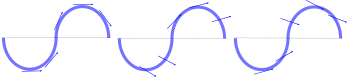
\includegraphics[width=0.9\columnwidth]{linICS_Inversion_Sketch_V2.pdf}
\caption{Inversion Sketch (Replace)}
\end{figure}
This leads to the next hypothesis which is that since we are interacting relatively far into the plasma the electron beam is still evolving and the transverse components still perform betatron oscillations. The betatron wavelength is given by
\begin{equation}
\lambda_\beta = \lambda_p \sqrt{2\gamma},
\end{equation}
with plasma wavelength
\begin{equation}
\lambda_p = n_e ...
\end{equation}
In this case for density XXX the plasma wavelength is XX and the betatron wavelength for a 1 GeV electron becomes XXX microns. The approximately remaining distance in the channel based on the shadowgraphy and the beam size is XX which means that the beam could change from one side to another in that time if it is around its maximum. However, the radiation is emitted in the direction of the momentum vector of the electrons. This means that in an oscillatory motion we would expect a distribution of emission angles and by chance sometimes an inverted but sometimes a non-inverted signal relation of the electron spectrum and the gamma profile. This is not being observed and the likelihood for this not to be seen for X shots is XXX. A consistent emission in the downwards trend would require that the betatron phase of the entire beam to be synchronised on every shot. Shock injection is able to produce narrow-energy spread and hence narrow-phase beams, but since we are measuring frequently spectrally long bunches we assume that extended injection events occurred. A fixed betatron phase, especially considering potentially varying shock positions, seems very unlikely.

Finally, the evolution of the wakefield could still point us into the right direction. The density profile measured interferometrically\footnote{Cary Colgan.} indicates a density spike at the edge of the channel. In this case we are shooting at 14 mm above the nozzle which is uncharacteristically high and supersonic nozzles are typically optimised for operation of a few mm above to guarantee a nice density plateau. The density profile is developing spikes at the edges, also without blade, at this height. A density up-ramp is associated to an increase in the focusing force the electrons experience in the bubble (REF). A long and high enough increase will force the electrons in any betatron phase back towards the axis and will turn their momentum vector to the centre. Density up-ramps have been proposed for rephasing and focusing of beams (REF). If the interaction occurs before the electrons moved another betatron phase to change sides then the interaction would produce an inverted gamma signal and a fixed betatron phase due to the focusing of the fields. The density profile is expected to remain roughly the same so the timing of the focusing would also be fixed, this seems more likely. 




\begin{figure}
\centering
\includegraphics[width=0.6\columnwidth]{RR19_02_11_r008_17-24_Average_density_cm3.png}
\caption[Interferometrically measured electron density of the plasma channel.]{Electron density in electrons per cm-3 in the plasma channel across the gas jet from 0 to 15 mm as measured interferometrically for a range of shots with the blade at the leading edge an without the scattering beam.}
\end{figure}

\begin{figure}
\centering

\includegraphics[width=0.9\columnwidth]{linICS_Inversion_Sketch_Bubble.pdf}
\caption[Sketch of how the momentum vectors of electrons at different phases in their betatron oscillations will be affected by a density transition.]{Sketch of how the momentum vectors of electrons at different phases in their betatron oscillations will be affected by a density transition. Following their oscillation first a density up-ramp leads to an increase of focusing fields which slowly directs the momentum vectors towards the centre as the electrons are pulled back stronger which increases further with density. The oscillations are now occurring at a new matched betatron wavelength. As the density decreases again, for instance at the end of the accelerator the focusing forces vanish and the electron beam diverges away from the axis.}
\end{figure}

At this stage a more extensive study and in particular a scan in timing or interaction plane would help to understand this behaviour better.
At the same time this indicates an interesting application of this diagnostic to investigate the beam dynamics in the plasma towards the end of the accelerator. Assuming the laser beam does not perturb the plasma significantly and both lasers arrive within a sufficiently small time window such that the ion motion does not become important. 
We can then use scans in time to investigate the orientation of the momentum vectors in the bubble as it approaches the end of the accelerator and determine when and how the freezing of the structures and the divergence of the beam is frozen into its structure. We could also use this to follow potential betatron oscillations through the accelerator giving us a snapshot of the beam dynamics at a given time.

On the other hand, in order to be a useful diagnostics for the beam parameters of the final electron beam and in order to be a useful pointing diagnostics or similar we have to be sure that we interact with the electron beam outside the plasma where the beam has fully evolved and does not change its shape, pointing or orientation any more.


\section{Conclusion}

In this Chapter we presented experimental results from linear inverse Compton scattering. We succeeded in colliding a relativistic electron beam from shock injection with a low intensity laser pulse producing consistently over hundreds of shots measurable gamma beams with radiation spectra consistent with linear inverse Compton scattering. Due to the variability of the electron beams produced in this setup the spectra of the gamma beams has been shown to vary from narrow-band 30 MeV radiation to broadband few to 30 MeV photon energies.

We also described a multi-shot procedure to estimate the laser beam size at the interaction and indicated how this can be used in a future radiation reaction study as alignment procedure to succeed in high-intensity laser collisions and to diagnose the interaction conditions.

We then discussed the application of linear inverse Compton scattering and in particular measuring the radiation profile as single-shot non-invasive electron beam diagnostic replacing a traditional beam profile and avoiding multi-shot techniques like the laser-wire.
The divergence measured from the gamma profile screen and the divergence of the electron beam in the non-dispersion axis were shown to be consistent with each other and the gamma profile measurement was then used to infer the ellipticity of the electron beam.
The analysis of the more detailed relation of the shape of the electron beam and the generated radiation indicated that the electron beam still evolved after the interaction resulting in a change in a global beam pointing and pointing of individual off-axis beamlets, which in particularly resulted in a relative to the vertical electron spectrum axis inverted gamma beam measurement. Linear ICS interactions hence promise to be an interesting diagnostic to study the beam dynamics at the end of the wakefield accelerator and study how the beam evolves until it freezes and diverges. This indicates that if this was to become a useful diagnostic of the final beam properties, the interaction plane has to be positioned outside of the plasma. The profile measurement also promises to become a useful tools in radiation reaction studies to determine the intensity at the interaction, but this also emphasises that the interaction has to occur at the end of the accelerator to allow for meaningful correlations.
